\documentclass{standalone}
\usepackage{tikz}
\usetikzlibrary{patterns, positioning}
\usepackage[sfdefault]{ClearSans} %% option 'sfdefault' activates Clear Sans as the default text font
\usepackage[T1]{fontenc}

\begin{document}
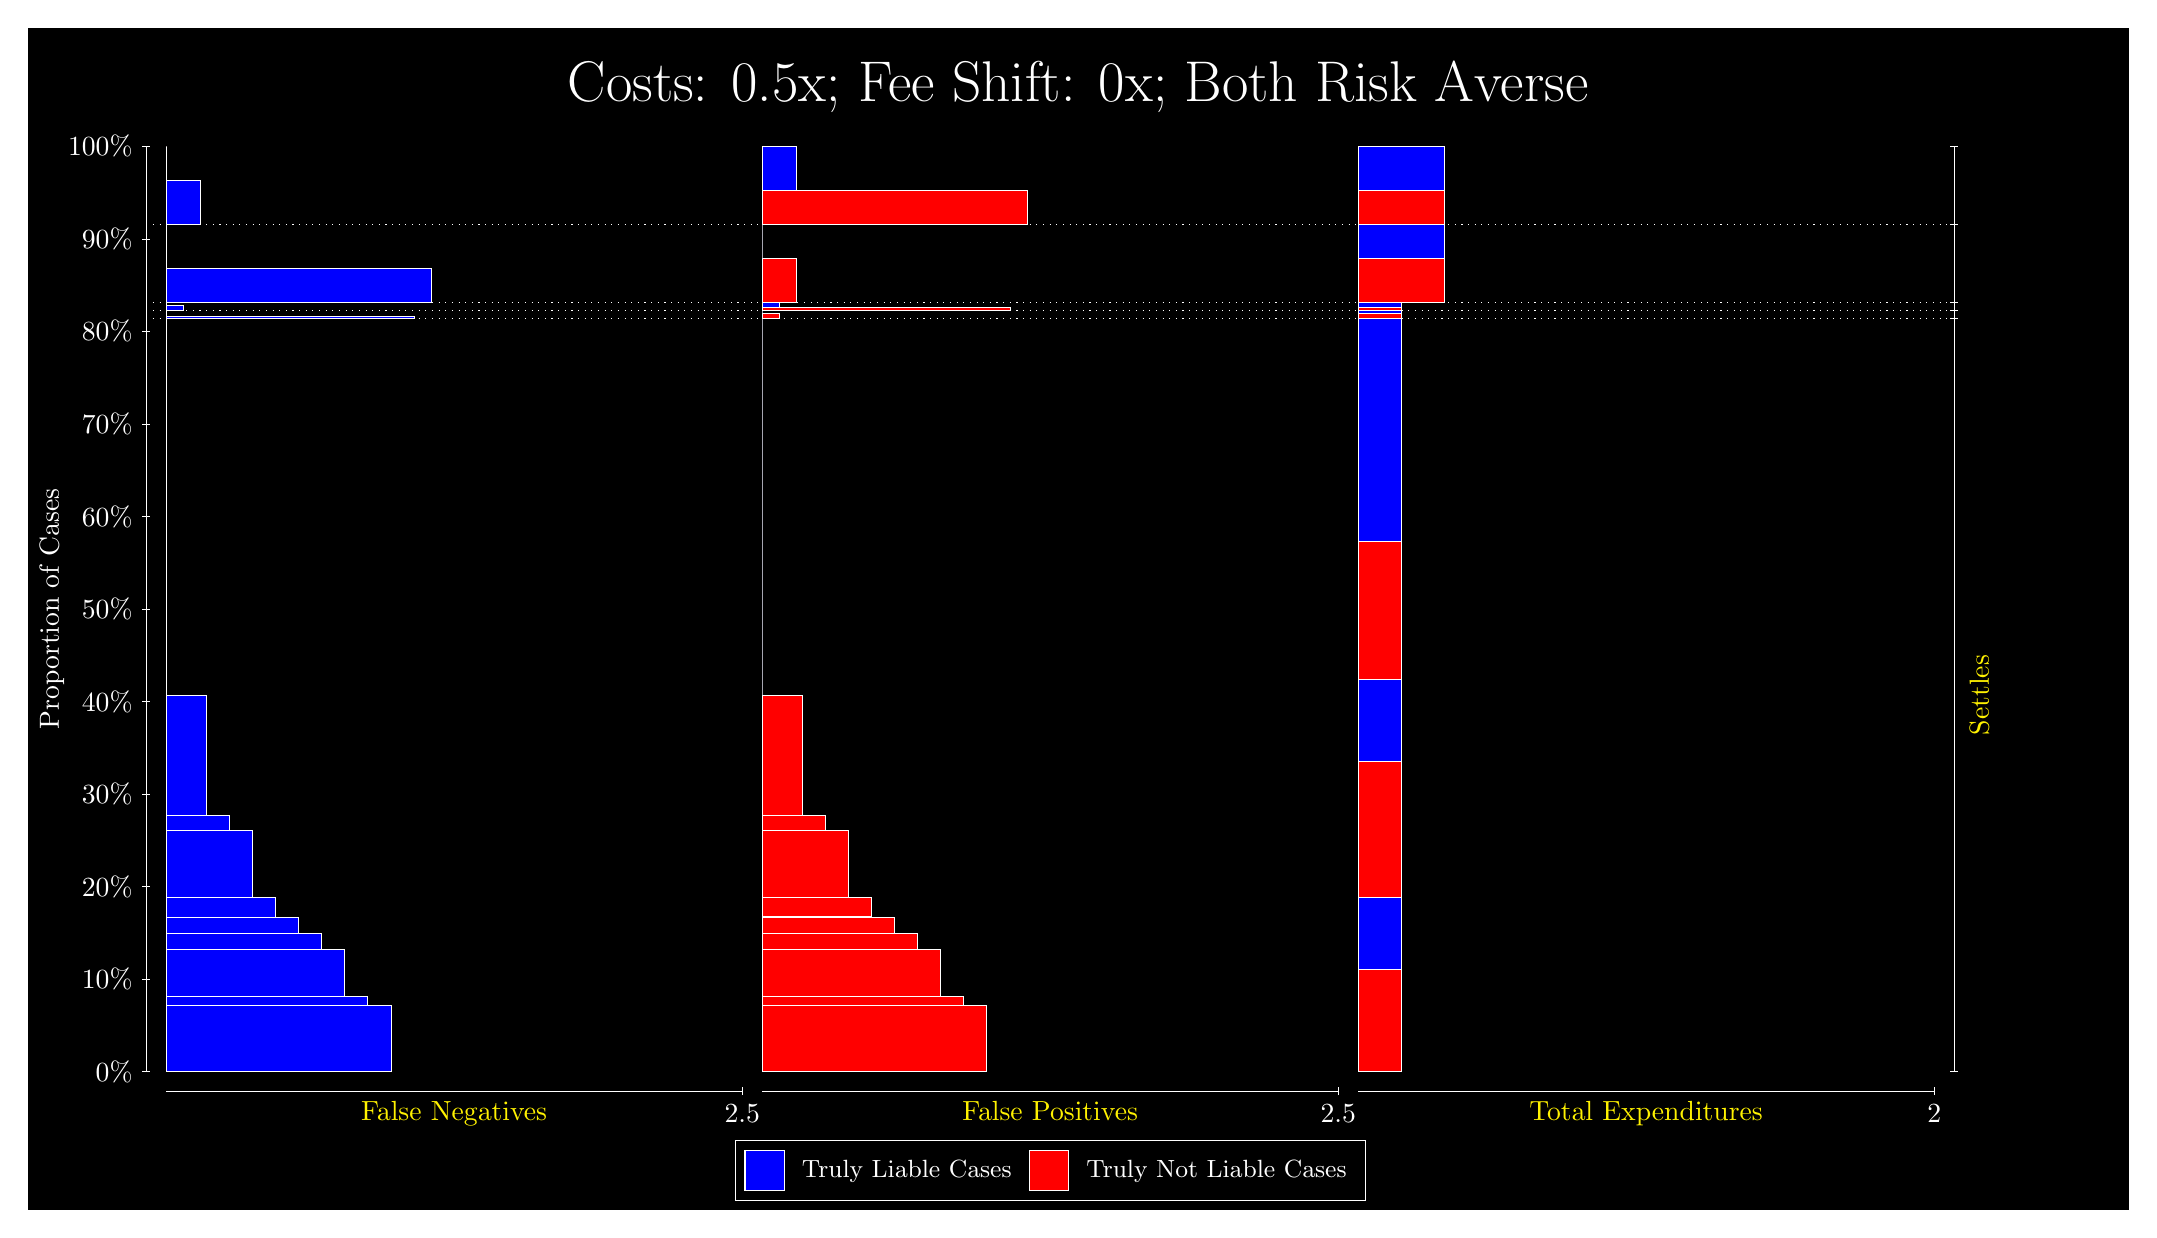
\begin{tikzpicture}
\draw[fill=black] (0,0) rectangle (26.667,15);
\draw[text=white] (0,13.5) rectangle (26.667,15) node[midway] {\huge Costs: 0.5x; Fee Shift: 0x; Both Risk Averse};
\draw[white, very thin] (1.5,1.75) -- (1.5,13.5);
\node[rotate=90, text=white, anchor=center] at (0.3, 7.625) {Proportion of Cases};
\draw[white, very thin] (1.45,1.75) -- (1.55,1.75);
\node[text=white, anchor=east] at (1.45, 1.75) {0\%};
\draw[white, very thin] (1.45,2.925) -- (1.55,2.925);
\node[text=white, anchor=east] at (1.45, 2.925) {10\%};
\draw[white, very thin] (1.45,4.1) -- (1.55,4.1);
\node[text=white, anchor=east] at (1.45, 4.1) {20\%};
\draw[white, very thin] (1.45,5.275) -- (1.55,5.275);
\node[text=white, anchor=east] at (1.45, 5.275) {30\%};
\draw[white, very thin] (1.45,6.45) -- (1.55,6.45);
\node[text=white, anchor=east] at (1.45, 6.45) {40\%};
\draw[white, very thin] (1.45,7.625) -- (1.55,7.625);
\node[text=white, anchor=east] at (1.45, 7.625) {50\%};
\draw[white, very thin] (1.45,8.8) -- (1.55,8.8);
\node[text=white, anchor=east] at (1.45, 8.8) {60\%};
\draw[white, very thin] (1.45,9.975) -- (1.55,9.975);
\node[text=white, anchor=east] at (1.45, 9.975) {70\%};
\draw[white, very thin] (1.45,11.15) -- (1.55,11.15);
\node[text=white, anchor=east] at (1.45, 11.15) {80\%};
\draw[white, very thin] (1.45,12.325) -- (1.55,12.325);
\node[text=white, anchor=east] at (1.45, 12.325) {90\%};
\draw[white, very thin] (1.45,13.5) -- (1.55,13.5);
\node[text=white, anchor=east] at (1.45, 13.5) {100\%};

\draw[white, very thin] (24.457,1.75) -- (24.457,13.5);
\draw[white, very thin] (24.407,1.75) -- (24.507,1.75);
\node[anchor=west] at (24.407, 1.75) {};
\draw[white, very thin] (24.407,11.311) -- (24.507,11.311);
\node[anchor=west] at (24.407, 11.311) {};
\draw[white, very thin] (24.407,11.415) -- (24.507,11.415);
\node[anchor=west] at (24.407, 11.415) {};
\draw[white, very thin] (24.407,11.519) -- (24.507,11.519);
\node[anchor=west] at (24.407, 11.519) {};
\draw[white, very thin] (24.407,12.509) -- (24.507,12.509);
\node[anchor=west] at (24.407, 12.509) {};
\draw[white, very thin] (24.407,13.5) -- (24.507,13.5);
\node[anchor=west] at (24.407, 13.5) {};

\draw[white, very thin, fill=blue] (1.75,1.75) rectangle (4.6044,2.5934);
\draw[white, very thin, fill=blue] (1.75,2.5934) rectangle (4.3116,2.7002);
\draw[white, very thin, fill=blue] (1.75,2.7002) rectangle (4.0188,3.298);
\draw[white, very thin, fill=blue] (1.75,3.298) rectangle (3.7261,3.5073);
\draw[white, very thin, fill=blue] (1.75,3.5073) rectangle (3.4333,3.7081);
\draw[white, very thin, fill=blue] (1.75,3.7081) rectangle (3.1406,3.9677);
\draw[white, very thin, fill=blue] (1.75,3.9677) rectangle (2.8478,4.8186);
\draw[white, very thin, fill=blue] (1.75,4.8186) rectangle (2.5551,5.0031);
\draw[white, very thin, fill=blue] (1.75,5.0031) rectangle (2.2623,6.5303);
\draw[white, very thin, fill=red] (1.75,6.5303) rectangle (1.75,11.311);
\draw[white, very thin, fill=blue] (1.75,11.311) rectangle (4.8971,11.347);
\draw[white, very thin, fill=red] (1.75,11.347) rectangle (1.75,11.415);
\draw[white, very thin, fill=blue] (1.75,11.415) rectangle (1.9696,11.483);
\draw[white, very thin, fill=red] (1.75,11.483) rectangle (1.75,11.519);
\draw[white, very thin, fill=blue] (1.75,11.519) rectangle (5.1167,11.953);
\draw[white, very thin, fill=red] (1.75,11.953) rectangle (1.75,12.509);
\draw[white, very thin, fill=blue] (1.75,12.509) rectangle (2.1891,13.066);
\draw[white, very thin, fill=red] (1.75,13.066) rectangle (1.75,13.5);
\draw[white, very thin, fill=red] (9.3189,1.75) rectangle (12.173,2.5934);
\draw[white, very thin, fill=red] (9.3189,2.5934) rectangle (11.88,2.7002);
\draw[white, very thin, fill=red] (9.3189,2.7002) rectangle (11.588,3.2979);
\draw[white, very thin, fill=red] (9.3189,3.2979) rectangle (11.295,3.5073);
\draw[white, very thin, fill=red] (9.3189,3.5073) rectangle (11.002,3.7081);
\draw[white, very thin, fill=red] (9.3189,3.7081) rectangle (10.709,3.7205);
\draw[white, very thin, fill=red] (9.3189,3.7205) rectangle (10.709,3.9677);
\draw[white, very thin, fill=red] (9.3189,3.9677) rectangle (10.417,4.8186);
\draw[white, very thin, fill=red] (9.3189,4.8186) rectangle (10.124,5.0031);
\draw[white, very thin, fill=red] (9.3189,5.0031) rectangle (9.8312,6.5304);
\draw[white, very thin, fill=blue] (9.3189,6.5304) rectangle (9.3189,11.311);
\draw[white, very thin, fill=red] (9.3189,11.311) rectangle (9.5384,11.378);
\draw[white, very thin, fill=blue] (9.3189,11.378) rectangle (9.3189,11.415);
\draw[white, very thin, fill=red] (9.3189,11.415) rectangle (12.466,11.451);
\draw[white, very thin, fill=blue] (9.3189,11.451) rectangle (9.5384,11.519);
\draw[white, very thin, fill=red] (9.3189,11.519) rectangle (9.758,12.075);
\draw[white, very thin, fill=blue] (9.3189,12.075) rectangle (9.3189,12.509);
\draw[white, very thin, fill=red] (9.3189,12.509) rectangle (12.686,12.944);
\draw[white, very thin, fill=blue] (9.3189,12.944) rectangle (9.758,13.5);
\draw[white, very thin, fill=red] (16.888,1.75) rectangle (17.437,3.045);
\draw[white, very thin, fill=blue] (16.888,3.045) rectangle (17.437,3.9589);
\draw[white, very thin, fill=red] (16.888,3.9589) rectangle (17.437,5.687);
\draw[white, very thin, fill=blue] (16.888,5.687) rectangle (17.437,6.7312);
\draw[white, very thin, fill=red] (16.888,6.7312) rectangle (17.437,8.4885);
\draw[white, very thin, fill=blue] (16.888,8.4885) rectangle (17.437,11.311);
\draw[white, very thin, fill=red] (16.888,11.311) rectangle (17.437,11.378);
\draw[white, very thin, fill=blue] (16.888,11.378) rectangle (17.437,11.415);
\draw[white, very thin, fill=red] (16.888,11.415) rectangle (17.437,11.451);
\draw[white, very thin, fill=blue] (16.888,11.451) rectangle (17.437,11.519);
\draw[white, very thin, fill=red] (16.888,11.519) rectangle (17.986,12.075);
\draw[white, very thin, fill=blue] (16.888,12.075) rectangle (17.986,12.509);
\draw[white, very thin, fill=red] (16.888,12.509) rectangle (17.986,12.944);
\draw[white, very thin, fill=blue] (16.888,12.944) rectangle (17.986,13.5);
\draw[white, dotted] (1.5,11.311) -- (24.457,11.311);
\draw[white, dotted] (1.5,11.415) -- (24.457,11.415);
\draw[white, dotted] (1.5,11.519) -- (24.457,11.519);
\draw[white, dotted] (1.5,12.509) -- (24.457,12.509);
\draw[white, very thin] (1.75,1.5) -- (9.0689,1.5);
\node[text=yellow, anchor=north] at (5.4094, 1.5) {False Negatives};
\draw[white, very thin] (9.0689,1.45) -- (9.0689,1.55);
\node[text=white, anchor=north] at (9.0689, 1.45) {2.5};

\draw[white, very thin] (9.3189,1.5) -- (16.638,1.5);
\node[text=yellow, anchor=north] at (12.978, 1.5) {False Positives};
\draw[white, very thin] (16.638,1.45) -- (16.638,1.55);
\node[text=white, anchor=north] at (16.638, 1.45) {2.5};

\draw[white, very thin] (16.888,1.5) -- (24.207,1.5);
\node[text=yellow, anchor=north] at (20.547, 1.5) {Total Expenditures};
\draw[white, very thin] (24.207,1.45) -- (24.207,1.55);
\node[text=white, anchor=north] at (24.207, 1.45) {2};

\node[text=yellow, centered, rotate=90] at (24.777, 6.5303) {Settles};





\draw (12.978300999999998,1.5) node[draw=none] (baseCoordinate) {};
\begin{scope}[align=center]
        \matrix[scale=0.5, draw=white, below=0.5cm of baseCoordinate, nodes={draw}, column sep=0.1cm]{
            \node[rectangle, draw, minimum width=0.5cm, minimum height=0.5cm, fill=blue] {}; &
            \node[draw=none, font=\small, text=white] (B) {Truly Liable Cases}; &
            \node[rectangle, draw, minimum width=0.5cm, minimum height=0.5cm, fill=red] {}; &
            \node[draw=none, font=\small, text=white] (B) {Truly Not Liable Cases}; \\
            };
\end{scope}

\end{tikzpicture}
\end{document}